%%%%%%%%%%%%%%%%%%%%%%%%%%%%%%%%%%%%%
%                                   %
% Compile with XeLaTeX and biber    %
%                                   %
% Questions or comments:            %
%                                   %
% joshua dot mcneill at uga dot edu %
%                                   %
%%%%%%%%%%%%%%%%%%%%%%%%%%%%%%%%%%%%%

\documentclass{beamer}
  % Read in standard preamble (cosmetic stuff)
  %%%%%%%%%%%%%%%%%%%%%%%%%%%%%%%%%%%%%%%%%%%%%%%%%%%%%%%%%%%%%%%%
% This is a standard preamble used in for all slide documents. %
% It basically contains cosmetic settings.                     %
%                                                              %
% Joshua McNeill                                               %
% joshua dot mcneill at uga dot edu                            %
%%%%%%%%%%%%%%%%%%%%%%%%%%%%%%%%%%%%%%%%%%%%%%%%%%%%%%%%%%%%%%%%

% Beamer settings
% \usetheme{Berkeley}
\usetheme{CambridgeUS}
% \usecolortheme{dove}
% \usecolortheme{rose}
\usecolortheme{seagull}
\usefonttheme{professionalfonts}
\usefonttheme{serif}
\setbeamertemplate{bibliography item}{}

% Packages and settings
\usepackage{fontspec}
  \setmainfont{Charis SIL}
\usepackage{hyperref}
  \hypersetup{colorlinks=true,
              allcolors=blue}
\usepackage{graphicx}
  \graphicspath{{../../figures/}}
\usepackage[normalem]{ulem}
\usepackage{enumerate}

% Document information
\author{M. McNeill}
\title[FREN2001]{Français 2001}
\institute{\url{joshua.mcneill@uga.edu}}
\date{}

%% Custom commands
% Lexical items
\newcommand{\lexi}[1]{\textit{#1}}
% Gloss
\newcommand{\gloss}[1]{`#1'}
\newcommand{\tinygloss}[1]{{\tiny`#1'}}
% Orthographic representations
\newcommand{\orth}[1]{$\langle$#1$\rangle$}
% Utterances (pragmatics)
\newcommand{\uttr}[1]{`#1'}
% Sentences (pragmatics)
\newcommand{\sent}[1]{\textit{#1}}
% Base dir for definitions
\newcommand{\defs}{../definitions}


  % Packages and settings

  % Document information
  \subtitle[Heures et verbes \lexi{-ir}]{Les heures et les verbes \lexi{-ir}}

\begin{document}
  % Read in the standard intro slides (title page and table of contents)
  \begin{frame}
    \titlepage
    \tiny{Office: % Basically a variable for office hours location
Gilbert 121\\
          Office hours: % Basically a variable for office hours
 lundi, mercredi, vendredi 10:10--11:10
}
  \end{frame}

  \begin{frame}{Les verbes \lexi{-ir}}
    Par example:
    \begin{center}
      \begin{tabular}{l | l l | l l}
  \multicolumn{5}{c}{dormir \gloss{to sleep}} \\
      & \multicolumn{2}{l |}{singulier} & \multicolumn{2}{l}{pluriel} \\
  \hline
  1re & je         & dors               & nous        & dormons \\
  2e  & tu         & dors               & vous        & dormez \\
  \hline
  3e  & il (masc)  &                    & ils (masc)  & \\
      & elle (fem) & dort               & elles (fem) & dorment \\
      & on         &                    &             & \\
\end{tabular}

    \end{center}
  \end{frame}

  \begin{frame}{Dans le monde francophone}
    Quelle heure est-il, et qu'est-ce qu'on fait...
    \only<1>{
      \begin{center}
        ... à la Nouvelle-Orléans?
      \end{center}
    }
    \only<2>{
      \begin{center}
        ... à Cayenne?
      \end{center}
    }
    \only<3>{
      \begin{center}
        ... à Dakar?
      \end{center}
    }
    \only<4>{
      \begin{center}
        ... à Marseille?
      \end{center}
    }
    \only<5>{
      \begin{center}
        ... à Djibouti?
      \end{center}
    }
    \only<6>{
      \begin{center}
        ... à Mahé?
      \end{center}
    }
    \only<7>{
      \begin{center}
        ... à Nouméa?
      \end{center}
    }
    \begin{center}
      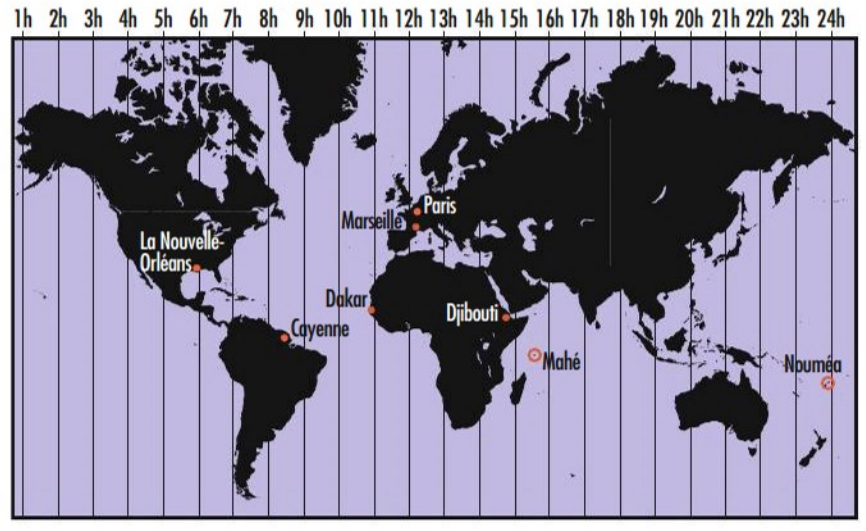
\includegraphics[scale=0.4]{heures.png}
    \end{center}
  \end{frame}

  \begin{frame}{}
    \begin{center}
      \Large Quiz
    \end{center}
  \end{frame}

  \begin{frame}{Trouver un/e colocataire}
    Avec un/e partenaire, comparez les heures où vous faites les activités suivantes.
    Est-ce que vous seriez de bons/bonnes colocataires? \\
    \tinygloss{With a partner, compare the times when you do the following activities.
    Would you be good roommates?}
    \begin{columns}
      \column{0.6\textwidth}
        \begin{description}
          \item[] \textbf{Modèle:}
          \item[] \lexi{se lever}
          \item[E1:] Normalement, je me lève à huit heures du matin. Et toi?
          \item[E2:] Moi, je me lève à dix heures, parce que mon premier cours et à onze heures et demi.
        \end{description}
      \column{0.4\textwidth}
        \small
        \begin{enumerate}
          \item se lever
          \item aller en cours
          \item faire du sport
          \item travailler
          \item manger le soir
          \item regarder la télé
          \item faire des devoirs
          \item se coucher
        \end{enumerate}
    \end{columns}
  \end{frame}

  \begin{frame}{Nos habitudes}
    \begin{columns}
      \column{0.5\textwidth}
        Circulez autour de la salle, et pour chaque description suivante, trouvez un/e camarade de classe à qui elle s'applique.
        Notez le nom de chaque personne. \\
        \tinygloss{Go around the room, and for each description below, find a classmate to whom it applies.
        Take note of the name of each person.}
      \column{0.5\textwidth}
        \begin{description}
          \item[] \textbf{Modèle:}
          \item[E1:] Est-ce que tu dors l'après-midi?
          \item[E2:] Oui, je dors à deux heures tous les jours.
        \end{description}
    \end{columns}
    \vspace{0.5cm}
    \begin{columns}[t]
      \scriptsize
      \column{0.5\textwidth}
        \begin{enumerate}
          \item s'endormir pendant les cours
          \item sortir pendant la semaine
          \item partir pour le week-end
          \item servir le dîner dans un restaurant
          \item dormir très tard le matin
        \end{enumerate}
      \column{0.5\textwidth}
        \begin{enumerate}
          \setcounter{enumi}{5}
          \item mentir quelquefois à ses parents
          \item partir de chez lui/elle très tôt le matin
          \item dormir l'après-midi
          \item partir en vacanes bientôt
          \item courir au parc le week-end
        \end{enumerate}
    \end{columns}
  \end{frame}

  \begin{frame}{}
    \begin{center}
      \Large Questions?
    \end{center}
  \end{frame}
\end{document}
